\documentclass{article}
\usepackage{fontspec}
\setsansfont{Helvetica}
\renewcommand{\familydefault}{\sfdefault}
\usepackage{tikz}
\usetikzlibrary{arrows.meta}
\pagestyle{empty}
\definecolor{cA}{HTML}{1F77B4}
\definecolor{cB}{HTML}{FF7F0E}
\definecolor{lookup}{HTML}{2A78D6}
\definecolor{lookuplight}{HTML}{9DC1EC}
\definecolor{write}{HTML}{EB6834}
\definecolor{writelight}{HTML}{F5B597}
\definecolor{ink}{HTML}{0B0B0B}
\definecolor{inktwo}{HTML}{52514E}
\definecolor{gridc}{HTML}{E4E3DF}
\definecolor{axisc}{HTML}{8F8E89}
\definecolor{refc}{HTML}{3D3C39}
\tikzset{
  tick/.style={font=\footnotesize, text=black, inner sep=1.5pt},
  lab/.style={font=\small, text=ink, inner sep=1.5pt},
  note/.style={font=\footnotesize, text=inktwo, inner sep=1.5pt},
  ser/.style={line width=1.4pt, line cap=round, line join=round},
  thin/.style={line width=0.9pt, line cap=round, line join=round},
  ref/.style={line width=0.8pt, draw=refc, dash pattern=on 3pt off 2pt},
}
\begin{document}
\setbox0=\hbox{%
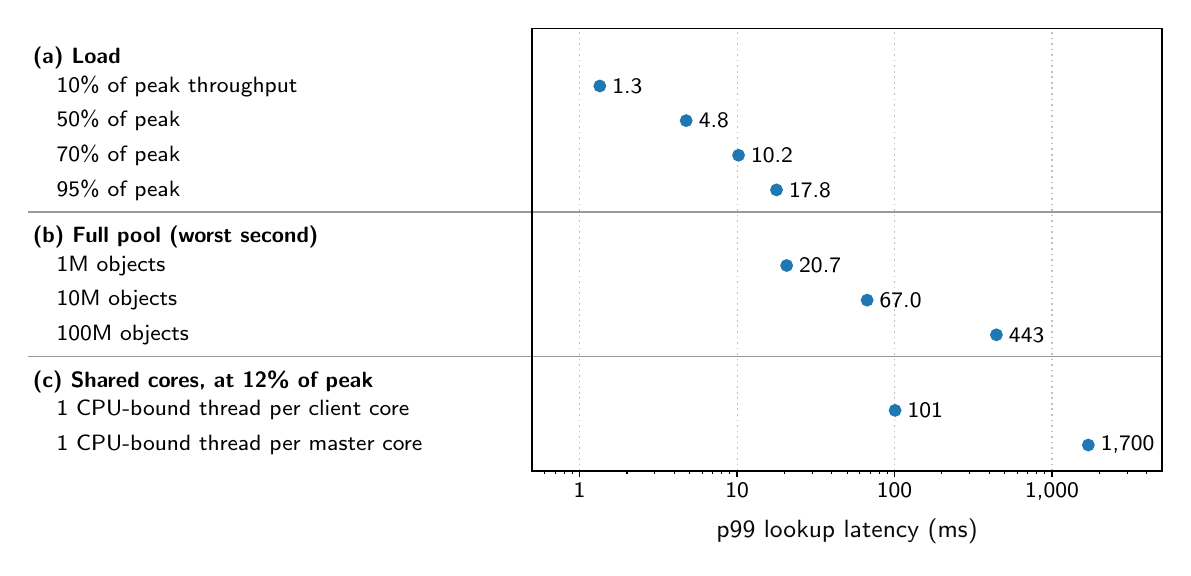
\begin{tikzpicture}[x=1cm,y=1cm]
\draw[black!25, line width=0.4pt, dash pattern=on 0.6pt off 1.4pt] (7.002,0.000) -- (7.002,5.620);
\draw[black, line width=0.6pt] (7.002,0.000) -- (7.002,-0.070);
\node[tick, anchor=north] at (7.002,-0.090) {1};
\draw[black!25, line width=0.4pt, dash pattern=on 0.6pt off 1.4pt] (9.002,0.000) -- (9.002,5.620);
\draw[black, line width=0.6pt] (9.002,0.000) -- (9.002,-0.070);
\node[tick, anchor=north] at (9.002,-0.090) {10};
\draw[black!25, line width=0.4pt, dash pattern=on 0.6pt off 1.4pt] (11.002,0.000) -- (11.002,5.620);
\draw[black, line width=0.6pt] (11.002,0.000) -- (11.002,-0.070);
\node[tick, anchor=north] at (11.002,-0.090) {100};
\draw[black!25, line width=0.4pt, dash pattern=on 0.6pt off 1.4pt] (13.002,0.000) -- (13.002,5.620);
\draw[black, line width=0.6pt] (13.002,0.000) -- (13.002,-0.070);
\node[tick, anchor=north] at (13.002,-0.090) {1,000};
\draw[black, line width=0.4pt] (6.558,0.000) -- (6.558,-0.040);
\draw[black, line width=0.4pt] (6.692,0.000) -- (6.692,-0.040);
\draw[black, line width=0.4pt] (6.808,0.000) -- (6.808,-0.040);
\draw[black, line width=0.4pt] (6.911,0.000) -- (6.911,-0.040);
\draw[black, line width=0.4pt] (7.604,0.000) -- (7.604,-0.040);
\draw[black, line width=0.4pt] (7.956,0.000) -- (7.956,-0.040);
\draw[black, line width=0.4pt] (8.206,0.000) -- (8.206,-0.040);
\draw[black, line width=0.4pt] (8.400,0.000) -- (8.400,-0.040);
\draw[black, line width=0.4pt] (8.558,0.000) -- (8.558,-0.040);
\draw[black, line width=0.4pt] (8.692,0.000) -- (8.692,-0.040);
\draw[black, line width=0.4pt] (8.808,0.000) -- (8.808,-0.040);
\draw[black, line width=0.4pt] (8.911,0.000) -- (8.911,-0.040);
\draw[black, line width=0.4pt] (9.604,0.000) -- (9.604,-0.040);
\draw[black, line width=0.4pt] (9.956,0.000) -- (9.956,-0.040);
\draw[black, line width=0.4pt] (10.206,0.000) -- (10.206,-0.040);
\draw[black, line width=0.4pt] (10.400,0.000) -- (10.400,-0.040);
\draw[black, line width=0.4pt] (10.558,0.000) -- (10.558,-0.040);
\draw[black, line width=0.4pt] (10.692,0.000) -- (10.692,-0.040);
\draw[black, line width=0.4pt] (10.808,0.000) -- (10.808,-0.040);
\draw[black, line width=0.4pt] (10.911,0.000) -- (10.911,-0.040);
\draw[black, line width=0.4pt] (11.604,0.000) -- (11.604,-0.040);
\draw[black, line width=0.4pt] (11.956,0.000) -- (11.956,-0.040);
\draw[black, line width=0.4pt] (12.206,0.000) -- (12.206,-0.040);
\draw[black, line width=0.4pt] (12.400,0.000) -- (12.400,-0.040);
\draw[black, line width=0.4pt] (12.558,0.000) -- (12.558,-0.040);
\draw[black, line width=0.4pt] (12.692,0.000) -- (12.692,-0.040);
\draw[black, line width=0.4pt] (12.808,0.000) -- (12.808,-0.040);
\draw[black, line width=0.4pt] (12.911,0.000) -- (12.911,-0.040);
\draw[black, line width=0.4pt] (13.604,0.000) -- (13.604,-0.040);
\draw[black, line width=0.4pt] (13.956,0.000) -- (13.956,-0.040);
\draw[black, line width=0.4pt] (14.206,0.000) -- (14.206,-0.040);
\node[tick, anchor=west, font=\footnotesize\bfseries] at (0,5.250) {(a) Load};
\node[tick, anchor=west] at (0.3,4.890) {10\% of peak throughput};
\filldraw[fill=cA, draw=cA, line width=0.8pt] (7.259,4.890) circle (1.9pt);
\node[tick, anchor=west] at (7.359,4.890) {1.3};
\node[tick, anchor=west] at (0.3,4.450) {50\% of peak};
\filldraw[fill=cA, draw=cA, line width=0.8pt] (8.356,4.450) circle (1.9pt);
\node[tick, anchor=west] at (8.456,4.450) {4.8};
\node[tick, anchor=west] at (0.3,4.010) {70\% of peak};
\filldraw[fill=cA, draw=cA, line width=0.8pt] (9.021,4.010) circle (1.9pt);
\node[tick, anchor=west] at (9.121,4.010) {10.2};
\node[tick, anchor=west] at (0.3,3.570) {95\% of peak};
\filldraw[fill=cA, draw=cA, line width=0.8pt] (9.503,3.570) circle (1.9pt);
\node[tick, anchor=west] at (9.603,3.570) {17.8};
\draw[black!40, line width=0.4pt] (0,3.290) -- (14.400,3.290);
\node[tick, anchor=west, font=\footnotesize\bfseries] at (0,2.970) {(b) Full pool (worst second)};
\node[tick, anchor=west] at (0.3,2.610) {1M objects};
\filldraw[fill=cA, draw=cA, line width=0.8pt] (9.632,2.610) circle (1.9pt);
\node[tick, anchor=west] at (9.732,2.610) {20.7};
\node[tick, anchor=west] at (0.3,2.170) {10M objects};
\filldraw[fill=cA, draw=cA, line width=0.8pt] (10.654,2.170) circle (1.9pt);
\node[tick, anchor=west] at (10.754,2.170) {67.0};
\node[tick, anchor=west] at (0.3,1.730) {100M objects};
\filldraw[fill=cA, draw=cA, line width=0.8pt] (12.296,1.730) circle (1.9pt);
\node[tick, anchor=west] at (12.396,1.730) {443};
\draw[black!40, line width=0.4pt] (0,1.450) -- (14.400,1.450);
\node[tick, anchor=west, font=\footnotesize\bfseries] at (0,1.130) {(c) Shared cores, at 12\% of peak};
\node[tick, anchor=west] at (0.3,0.770) {1 CPU-bound thread per client core};
\filldraw[fill=cA, draw=cA, line width=0.8pt] (11.009,0.770) circle (1.9pt);
\node[tick, anchor=west] at (11.109,0.770) {101};
\node[tick, anchor=west] at (0.3,0.330) {1 CPU-bound thread per master core};
\filldraw[fill=cA, draw=cA, line width=0.8pt] (13.463,0.330) circle (1.9pt);
\node[tick, anchor=west] at (13.563,0.330) {1,700};
\draw[black, line width=0.6pt] (6.400,0.000) rectangle (14.400,5.620);
\node[lab, anchor=north] at (10.400,-0.55) {p99 lookup latency (ms)};
\end{tikzpicture}}%
\pdfvariable horigin=0pt
\pdfvariable vorigin=0pt
\pagewidth=\dimexpr\wd0+8pt\relax
\pageheight=\dimexpr\ht0+\dp0+8pt\relax
\shipout\vbox{\kern4pt\hbox{\kern4pt\box0\kern4pt}\kern4pt}
\end{document}
